\documentclass[aspectratio=169]{beamer}
\usepackage[utf8]{inputenc}
\usepackage{amsmath,amssymb}
\usepackage{graphicx}
\usepackage{tikz}
\usetikzlibrary{shapes,arrows,positioning,calc}
\usepackage{hyperref}
\usepackage{xcolor}

% Custom 3B1B-inspired color palette
\definecolor{darkblue}{RGB}{10, 25, 47}
\definecolor{midblue}{RGB}{28, 73, 110}
\definecolor{lightcyan}{RGB}{116, 192, 227}
\definecolor{brownweight}{RGB}{140, 98, 57}
\definecolor{textgray}{RGB}{40, 40, 40}
\definecolor{bglight}{RGB}{248, 249, 250}

\setbeamercolor{palette primary}{bg=darkblue,fg=white}
\setbeamercolor{palette secondary}{bg=midblue,fg=white}
\setbeamercolor{palette tertiary}{bg=lightcyan,fg=darkblue}
\setbeamercolor{structure}{fg=midblue}
\setbeamercolor{background canvas}{bg=bglight}
\setbeamercolor{normal text}{fg=textgray}

\setbeamertemplate{navigation symbols}{}
\setbeamertemplate{footline}{
  \hfill\usebeamercolor[fg]{page number in head/foot}\usebeamerfont{page number in head/foot}
  \insertframenumber\,/\,\inserttotalframenumber\kern2em\vskip2pt
}

\title{Lecture 3: The Attention Mechanism Step-by-Step}
\subtitle{Queries, Keys, Values, and Multi-Head Attention}
\author{Transformer Lectures Series}
\date{Based on 3Blue1Brown Lessons}

\begin{document}

% Slide 1: Title Slide
\begin{frame}[plain]
  \titlepage
\end{frame}

% Slide 2: Motivation: Context and Ambiguity
\begin{frame}{Why Attention? The Polysemy Problem}
  Standard dictionary definitions do not define a word's usage in a specific phrase:
  
  \begin{exampleblock}{The Word "Mole"}
    \begin{itemize}
      \item "American shrew \textbf{mole}" $\rightarrow$ Mammal/Animal
      \item "One \textbf{mole} of carbon dioxide" $\rightarrow$ Chemical Quantity
      \item "Take a biopsy of the \textbf{mole}" $\rightarrow$ Dermatological/Skin condition
    \end{itemize}
  \end{exampleblock}
  
  \begin{itemize}
    \item \textbf{Goal}: Embeddings must absorb contextual information from surrounding words.
    \item E.g., The vector for "mole" must absorb information from "shrew" or "biopsy".
  \end{itemize}
\end{frame}

% Slide 3: Information Flow in Attention
\begin{frame}{Information Flow: Shifting Vectors}
  \centering
  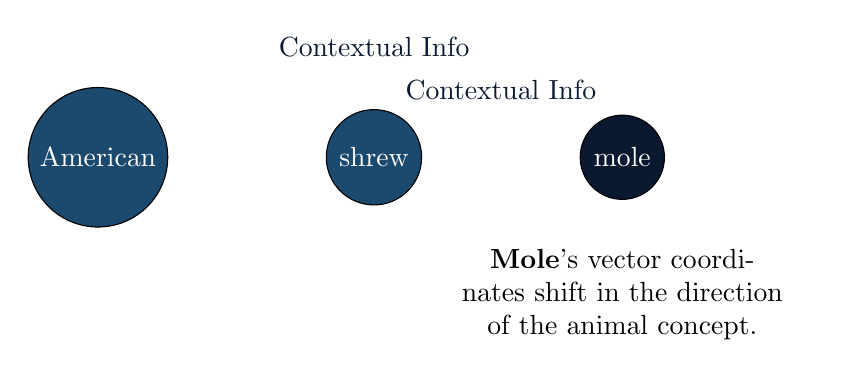
\begin{tikzpicture}[node distance=2cm, auto, >=latex]
    \node[draw, circle, fill=midblue, text=white] (t1) {American};
    \node[draw, circle, fill=midblue, text=white, right=of t1] (t2) {shrew};
    \node[draw, circle, fill=darkblue, text=white, right=of t2] (t3) {mole};
    
    \path[->, thick, darkblue, dashed] (t1) to[bend left] node[above] {Contextual Info} (t3);
    \path[->, thick, darkblue, dashed] (t2) to[bend left] node[above] {Contextual Info} (t3);
    
    \node[below=0.5cm of t3, text width=5cm, text centered] {
      \textbf{Mole}'s vector coordinates shift in the direction of the animal concept.
    };
  \end{tikzpicture}
\end{frame}

% Slide 4: Queries, Keys, and Values
\begin{frame}{Queries, Keys, and Values: The Core Concept}
  For any token vector $x_i$, we project it into three distinct roles:
  
  \begin{itemize}
    \item \textbf{Query ($q_i \in \mathbb{R}^k$)}: "What am I looking for?"
      \begin{itemize}
        \item Projected using weight matrix $W_Q$: $q_i = W_Q x_i$
      \end{itemize}
    \item \textbf{Key ($k_j \in \mathbb{R}^k$)}: "What information do I offer?"
      \begin{itemize}
        \item Projected using weight matrix $W_K$: $k_j = W_K x_j$
      \end{itemize}
    \item \textbf{Value ($v_j \in \mathbb{R}^v$)}: "What content do I actually transfer?"
      \begin{itemize}
        \item Projected using weight matrix $W_V$: $v_j = W_V x_j$
      \end{itemize}
  \end{itemize}
\end{frame}

% Slide 5: Math Step 1: Attention Scores (Compatibility)
\begin{frame}{Math Step 1: Calculating Alignment}
  How much should token $i$ pay attention to token $j$? We measure this by the dot product of the Query of $i$ and Key of $j$:
  
  \[
  \text{Score}_{ij} = q_i \cdot k_j = q_i^T k_j
  \]
  
  \begin{itemize}
    \item A high score indicates that what token $i$ is looking for aligns with what token $j$ offers.
    \item \textbf{Scaling}: To prevent variance from blowing up in high dimensions (which leads to vanishing gradients in Softmax), we divide by the square root of the key dimension $\sqrt{d_k}$:
      \[
      \text{Scaled Score}_{ij} = \frac{q_i^T k_j}{\sqrt{d_k}}
      \]
  \end{itemize}
\end{frame}

% Slide 6: Causal Masking: Keeping the Future Secret
\begin{frame}{Causal Masking (Autoregressive Generation)}
  In a generative model (like GPT), tokens are not allowed to attend to future tokens.
  
  \begin{columns}
    \begin{column}{0.5\textwidth}
      \begin{itemize}
        \item We apply a \textbf{mask} to the score matrix.
        \item Future positions (where $j > i$) are set to $-\infty$ before applying Softmax:
          \[
          \text{Masked Score}_{ij} = 
          \begin{cases} 
            \frac{q_i^T k_j}{\sqrt{d_k}} & \text{if } j \le i \\
            -\infty & \text{if } j > i
          \end{cases}
          \]
        \item Since $e^{-\infty} = 0$, future tokens receive exactly 0 attention weight.
      \end{itemize}
    \end{column}
    
    \begin{column}{0.5\textwidth}
      \centering
      \textbf{Attention Mask Matrix}
      \[
      \begin{pmatrix}
        s_{11} & -\infty & -\infty & -\infty \\
        s_{21} & s_{22} & -\infty & -\infty \\
        s_{31} & s_{32} & s_{33} & -\infty \\
        s_{41} & s_{42} & s_{43} & s_{44}
      \end{pmatrix}
      \]
    \end{column}
  \end{columns}
\end{frame}

% Slide 7: Math Step 2: Softmax & The Attention Weights
\begin{frame}{Math Step 2: Softmax & Value Summation}
  Once scores are scaled and masked, we apply Softmax to get the final attention weights $A_{ij}$:
  
  \[
  A_{ij} = \text{Softmax}\left( \text{Scores}_i \right)_j = \frac{e^{\text{Score}_{ij}}}{\sum_k e^{\text{Score}_{ik}}}
  \]
  
  These weights represent the percentage of information to pull from each source.
  We then sum the Value vectors weighted by $A_{ij}$:
  
  \[
  u_i = \sum_{j} A_{ij} v_j
  \]
  
  $u_i$ is the compiled contextual update for token $i$.
\end{frame}

% Slide 8: The Output Projection
\begin{frame}{Step 3: Writing Back to the Residual Stream}
  The compiled update vector $u_i$ is mapped back into the main residual stream space:
  
  \[
  \Delta x_i = W_O u_i
  \]
  
  where $W_O$ is the **Output Projection** matrix.
  
  \begin{itemize}
    \item \textbf{Residual Addition}: The adjustment is added back directly:
      \[
      x_{i,\text{next}} = x_{i,\text{prev}} + \Delta x_i
      \]
    \item The original vector is preserved, but its semantic orientation is now updated with context.
  \end{itemize}
\end{frame}

% Slide 9: Multi-Head Attention
\begin{frame}{Multi-Head Attention: Parallel Relationships}
  A single attention operation (a "head") can only look for one type of context at a time.
  
  \begin{itemize}
    \item \textbf{The Solution}: Run multiple independent attention heads in parallel.
    \item Each head has its own $W_Q, W_K, W_V$ matrices:
      \begin{itemize}
        \item **Head 1**: Looks for adjective-noun pairings.
        \item **Head 2**: Looks for pronouns and their references.
        \item **Head 3**: Looks for subject-verb alignments.
      \end{itemize}
    \item \textbf{Aggregation}: The outputs of all heads are concatenated together and multiplied by $W_O$ to be written back to the residual stream.
  \end{itemize}
\end{frame}

% Slide 10: Attention Block Parameter Counts
\begin{frame}{Parameter Count in a Single Block}
  Let's estimate the size of a single Multi-Head Attention layer in GPT-3:
  \begin{itemize}
    \item Input dimension $d = 12,288$.
    \item $N_{\text{heads}} = 96$. Each head projects down to dimension $d_{\text{head}} = 12,288 / 96 = 128$.
    \item For each head:
      \begin{itemize}
        \item $W_Q, W_K, W_V \in \mathbb{R}^{d \times d_{\text{head}}}$. Total weights per head = $3 \times 12,288 \times 128 \approx 4.7$ million.
      \end{itemize}
    \item Stacking all 96 heads: $\approx 450$ million weights.
    \item Plus the output matrix $W_O \in \mathbb{R}^{d \times d}$: $12,288 \times 12,288 \approx 150$ million weights.
    \item **Total parameters per layer**: $\approx 600$ million parameters!
  \end{itemize}
\end{frame}

% Slide 11: Summary
\begin{frame}{Summary: Lecture 3 Recap}
  \begin{itemize}
    \item **Polysemy** requires token vectors to dynamically absorb surrounding context.
    \item **Queries ($Q$)** represent requests, **Keys ($K$)** represent contents, and **Values ($V$)** represent payloads.
    \item **Attention Scores** are calculated via scaled dot-product and causal masking.
    \item Multi-Head Attention runs multiple operations in parallel to map different types of linguistic interactions.
  \end{itemize}
\end{frame}

\end{document}
